% !TeX spellcheck = la_LA
% !TeX encoding = UTF-8
\documentclass[10pt]{article}

% A LaTeX reproduction of "Observationes Cyclometricae" by A.A. Kochanski,
%
% Typeset by Daniel Delimata

\usepackage[
    paperwidth=15.02cm,
    paperheight=20.33cm,
    left=9mm,
    right=40.5mm,
    top=13mm,
    bottom=0mm
    ]{geometry}
\pagestyle{empty}
\setlength{\parindent}{8.2mm}

\usepackage{microtype}
\usepackage[T1]{fontenc}

\usepackage{fontspec}
\setmainfont{IM FELL DW Pica PRO}

\usepackage{lettrine}
\usepackage{calc}
\usepackage{tikz}
\usetikzlibrary{intersections,calc}
\usepackage{wrapfig}
\usepackage{wallpaper}

\begin{document}%
\TileWallPaper{0.5\textwidth}{0.5\textheight}{paper_background.jpg}

    \font\1="IM FELL DW Pica PRO:mapping=tex-text,+dlig,+hlig,+hist" at 11pt
    \1
%----------------------------------------------------------------------
\noindent\hfill {\large \,\,\,\,\,MENSIS AUGUSTI\, A.\, M\, DC\, LXXXV. \hfill 
397}\smallskip

Colligitur ex eadem secundo.\, Rationes a nobis exhibitas\,, ad-\linebreak
eo compendiosas esse, ut earum nonnullæ\,, duplo pluribus notis Ar-\linebreak
chimedeis æquivaleant\,; quanquam ipsa Cc duplum earum excedat,\linebreak
quæ proinde brevitate\,, nec non exactitudine sua\,, in Praxi cæte-\linebreak
ris præferenda videatur\,, cui\,, dum quid accuratius quæritur\,,\, ipsa 
d\linebreak
succedat.\, Præter has quidem mihi suppetunt adhuc plures, consi-\linebreak
mili dote præditæ\,, sed eas,ne nimius videar\,, alteri occasioni 
servan-\linebreak
das existimo. Concludam interim singulari quadam, \& ut ita dicam,\linebreak
curiosa Ratione\,, quæ est 991 ad 
3113$\frac{\textrm{991}}{\textrm{3113}}$,
quæ cum Archimedea con-\vspace*{-4pt}\linebreak
sentit in octonis notis prioribus\,, ac tum primum illam incipit exce-\linebreak
dere\,, minus quam 23 centesimis.\medskip

\begin{centering}
\large \scalebox{1.0}[1]{\textit{GRAMMICÆ\,\,\, RATIONES\,\,\, CYCLOMETRICÆ,}}

\large \scalebox{1.0}[1]{\textit{Ad Uſus Mechanicos.}}

\end{centering}
\lettrine[lines=2, loversize=0.33, nindent=0pt]{H}{}%
\hspace*{-2.5pt}Arum\,quidem\,complures\,olim\,a\,me\,repertæ;hoc\,tamen\,loco\,vi\-sum
mihi est eam tantum proponere\,, quæ huic Anno præsenti,\linebreak
quo ista scribimus,affinitate quadam conjuncta est.

Oporteat igitur Semiperipheriæ B\,C\,D Rectam proxime æqua-\linebreak
lem reperire.\, Ducantur Tangentes BG,DH, quarum prior Radio\linebreak
AC æqualis, \& jungantur GCH. Tum Radio CA secentur ex C arcus\linebreak
utrinque æquales CE \& EF\,: quorum quivis complectetur Gradus\linebreak
60, reliqui autem BE, DF singuli gr. 30.{\,} Agatur per E Secans\linebreak
AI, determinans Tangentem BI. Capiatur tandem HL\,, æqualis\linebreak
Diametro BD\,; ac tum ducatur IL. \vspace{-0.7\baselineskip}

\begin{wrapfigure}[4]{l}{4cm}\,\small
    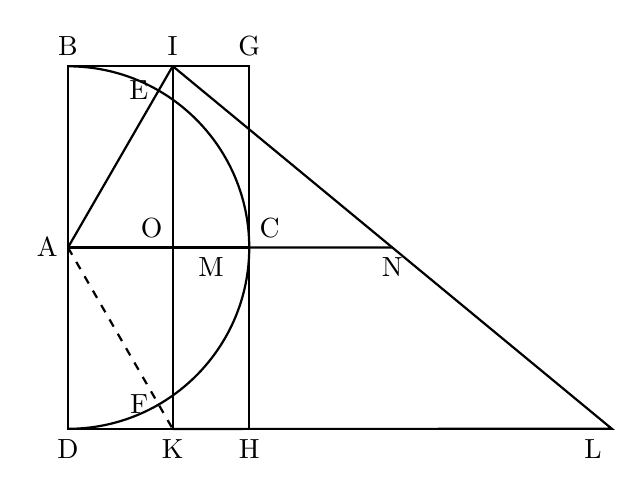
\begin{tikzpicture}[scale=1.151,thick]
    \coordinate (A) at (0,0);
    \coordinate (B) at (0,2);
    \coordinate (G) at (2,2);
    \coordinate (C) at (2,0);
    \coordinate (D) at (0,-2);
    \coordinate (H) at (2,-2);
    \coordinate (L) at (6,-2);
    \draw (A) node[left] {A}
        -- (B) node[above] {B}
        -- (G) node[above] {G}
        -- (C) node[above right] {C}
        -- (A)
        -- (D) node[below] {D}
        -- (H) node[below] {H}
        -- (C);
    \draw (D) arc(-90:90:2);
    \path [name path=BG line] (B) -- (G);
    \path [name path=AE line] (A) -- (60:2.4);
    \draw [name intersections={of=BG line and AE line, by=I}]
        (A) -- (I) node [above] {I};
    \path [name path=DH line] (D) -- (H);
    \path [name path=AF line] (A) -- (-60:2.4);
    \draw [dashed,name intersections={of=DH line and AF line, by=K}]
        (A) -- (K) node [below] {K};
    \draw [name path=IK line](I) -- (K);
    \path [name path=AC line](A) -- (C);
    \draw [name intersections={of=IK line and AC line, by=O}]
        (O) node [above left] {O};
    \draw (60:2) node [left] {E};
    \draw (-60:2) node [left] {F};
    \draw (I)
        -- (L) node [below left] {L}
        -- (K);    
    \draw (C) -- ($(I)!0.5!(L)$) node [below] {N};
    \draw ($(O)!0.5!(C)$) node [below] {M};
\end{tikzpicture}
\end{wrapfigure}
\noindent\begin{flushright}\vspace{-0.4\baselineskip}
    Dico\, Inprimis\, IL\, æqualem esse\linebreak
    Semiperipheriæ BCD pro-\linebreak
    xime.\qquad\qquad\qquad\qquad\,\,
    
    Demonstratur\, calculo\, Trigo-\linebreak
    nometrico.\quad Intelligatur\linebreak
    autem ducta esse IK, quæ\linebreak
    Tangentes\, BI\,,\, DK\, con-\linebreak
    jungat.\qquad\quad\,\vspace{4\baselineskip}

Quo-
\end{flushright}
\newpage
\noindent
«The Fell Types are digitally reproduced by Igino Marini. www.iginomarini.com»
\end{document}
